\subsection{ソフトウェア設計プロセス}

ソフトウェア設計は、一般に多段階の活動として考えられる。段階は、常に厳密に分かれるわけではないが、何を決める段階かを理解すると、設計成果物を作りやすくなる。

設計は、三つの段階に分けられる。
\begin{itemize}
  \item アーキテクチャ設計：システム全体の根本的な構造、主要構成要素、接続方式、支配的な品質方針を決める。
  \item \term{高水準設計}{High-Level Design}：外部に向いた設計であり、主要構成要素と外部環境のやり取り、構成要素間のやり取りを決める。
  \item \term{詳細設計}{Detailed Design}：内部に向いた設計であり、構成要素の内部構造、データ構造、アルゴリズム、内部モジュールを決める。
\end{itemize}

段階の境界は、プロジェクトやシステムの性質で変わる。たとえば、通常ならプログラマが選ぶソートアルゴリズムでも、極端な性能要求があるシステムでは、初期の設計段階で決める必要がある。このように、何をいつ決めるかは、その判断が要求達成にどれほど重要かで決まる。

\par\smallskip
\begin{center}
\centering
\IfFileExists{assets/generated_figures/ch03/fig-ch03-05.png}{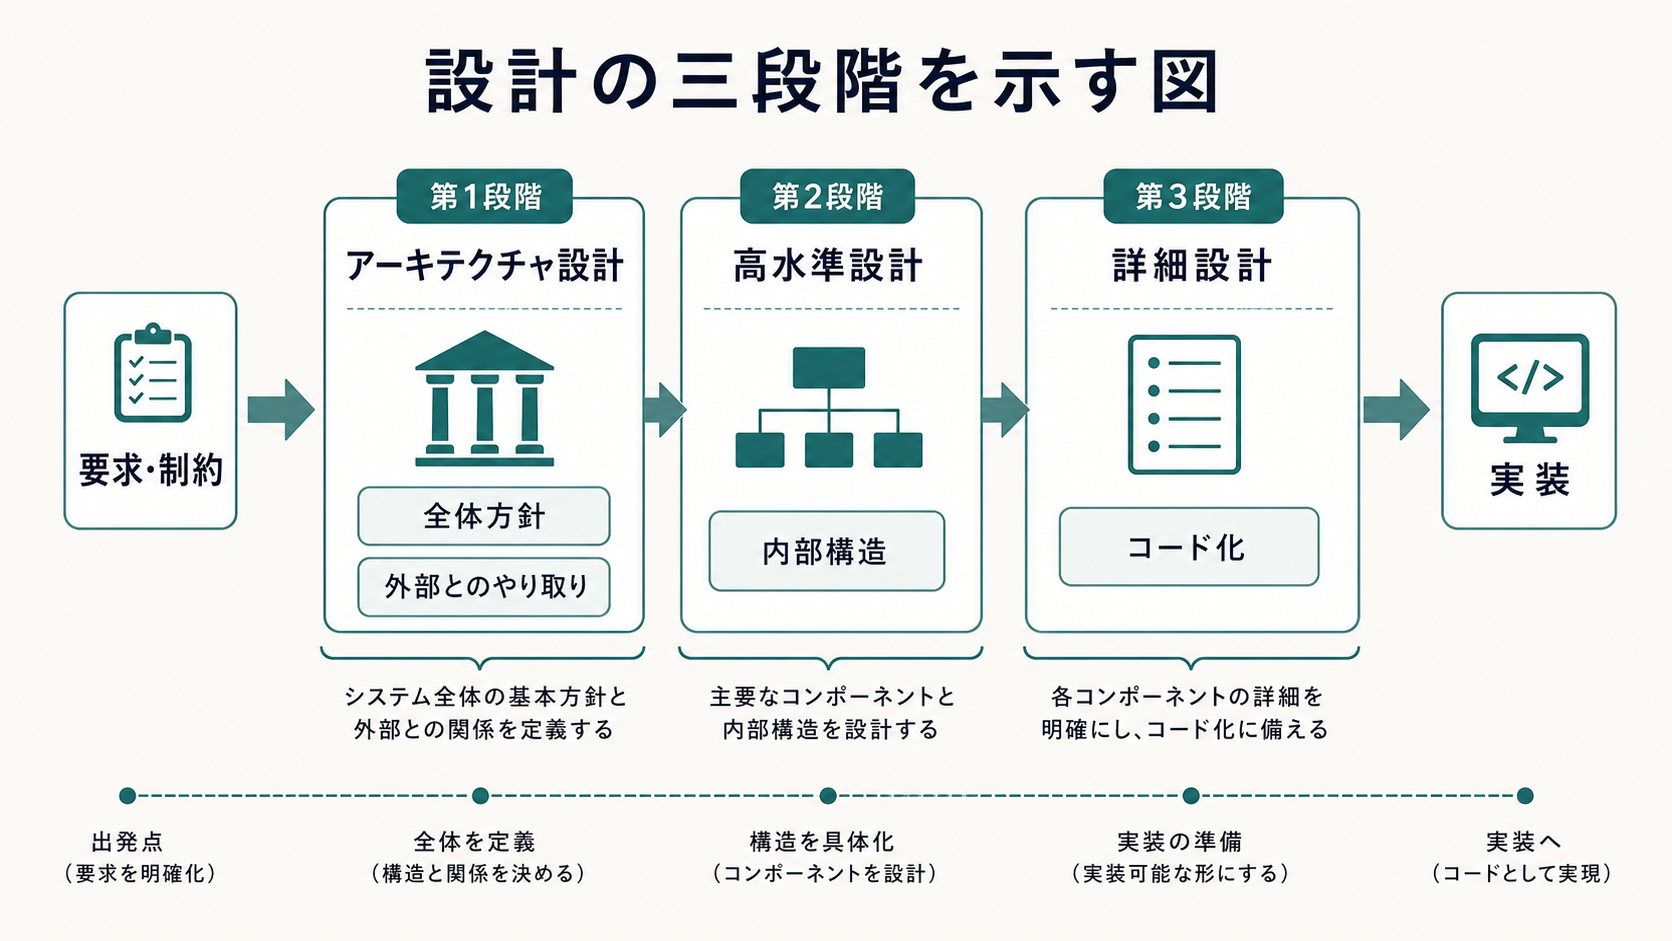
\includegraphics[width=0.96\linewidth]{assets/generated_figures/ch03/fig-ch03-05.png}}{\fbox{\parbox[c][48mm][c]{0.9\linewidth}{\centering 画像生成待ち\\設計の三段階を示す図}}}
\par\smallskip
\refstepcounter{figure}\label{fig:ch03-05}図 \thefigure: 設計の三段階を示す図
\end{center}
図 \thefigure は、設計の三段階を示す図を視覚的に整理したものである。
\par\smallskip

\subsubsection{高水準設計}

高水準設計 は、システムの主要構成要素が互いにどう関わり、外部環境とどうやり取りするかを決める設計である。外部環境には、利用者、外部システム、デバイス、ネットワーク、データベース、運用環境などが含まれる。

高水準設計では、主に次を扱う。
\begin{itemize}
  \item システムが反応すべき外部イベントやメッセージ。
  \item システムが生成すべきイベントやメッセージ。
  \item イベントやメッセージのデータ形式とプロトコル。
  \item 入力と出力の順序、タイミング、依存関係。
  \item 端から端までの取引やイベント列の流れ。
  \item データをどのように保存し、管理するか。
\end{itemize}

高水準設計は、アーキテクチャがある場合、その枠内で行われる。たとえば、アーキテクチャが「非同期メッセージでやり取りする」と決めていれば、高水準設計ではその方針に従って、具体的なメッセージ種類、順序、例外時の扱いを決める。

\subsubsection{詳細設計}

詳細設計 は、主要構成要素の内部を実装できる水準まで具体化する設計である。これは、プログラマがコードを書くための直接的な手がかりになる。

詳細設計では、主に次を扱う。
\begin{itemize}
  \item 主要構成要素を内部モジュールやプログラム単位へ分ける。
  \item 各モジュールの責務を割り当てる。
  \item モジュール間のやり取りを決める。
  \item 名前の有効範囲、可視性、公開・非公開の境界を決める。
  \item 状態、モード、状態遷移を定義する。
  \item データと制御の依存関係を明らかにする。
  \item データ構造、アルゴリズム、ユーザインタフェースの詳細を決める。
\end{itemize}

詳細設計は、実装と完全に分離して行われるとは限らない。特に反復型やアジャイル型の開発では、設計と実装が近い間隔で進む。しかし、その場合でも、設計判断が存在しなくなるわけではない。設計判断がコードの中だけに閉じ込められるのか、明示的に記録されるのかが変わるだけである。
